% !TEX encoding = UTF-8 Unicode

\documentclass[a4paper]{article}

\usepackage{color}
\usepackage{url}
\usepackage[T2A]{fontenc} % enable Cyrillic fonts
\usepackage[utf8]{inputenc} % make weird characters work
\usepackage{graphicx}
\usepackage[document]{ragged2e}
\usepackage{}
\usepackage[english,serbian]{babel}
\usepackage[
    style=numeric,
    sorting=none
]{biblatex}
\addbibresource{seminarski.bib}
\usepackage[table]{xcolor}

\usepackage[unicode]{hyperref}
\hypersetup{colorlinks,citecolor=green,filecolor=green,linkcolor=blue,urlcolor=blue}



\begin{document}
\title{Svemir kao velika neuronska mreža\\ \small{Seminarski rad u okviru kursa\\Tehničko i naučno pisanje\\ Matematički fakultet}}

\author{
    Filipović, Aleksa\\ 
    mi22139@alas.matf.bg.ac.rs
    \and
    Kiso, Marta\\ 
    mi22152@alas.matf.bg.ac.rs
    \and
    Seničanin, Veljko\\ 
    mi22252@alas.matf.bg.ac.rs
    \and
    Stamenković, Luka\\ 
    mi22271@alas.matf.bg.ac.rs
}
\date{15.~novembar 2022.}
\maketitle
\abstract{\justifying{
U ovom radu ćemo diskutovati o mogućnosti da je ceo univerzum jedna velika neuronska mreža. Samu ideju je dao ruski naučnik Vitali Vančurin sa Univerziteta u Minesoti u svom naučnom radu \cite{1}.
\\Princip kog ćemo pokušati da se držimo jeste taj da ne zalazimo previše u oblasti fizike i astronomije, već da na što jednostavniji način pokušamo da približimo ovu temu čitaocima. Opisaćemo šta je to neuronska mreža, kao i da li i na koji način je možemo povezati sa kosmososom.
}}
\tableofcontents

\newpage

\section{Uvod}
\label{sec:uvod}
\justifying
Kako bismo uopšte mogli da razmatramo opciju da se svemir može zamisliti kao neuronska mreža, važno je da tačno definišemo šta je to neuronska mreža. U uvodu ćemo je posmatrati iz biološkog ugla, dok ćemo u narednom poglavlju diskutovati o neuronskoj mreži u vidu implementacije sistema veštačke inteligencije. Neuronska mreža predstavlja nervni sistem živih bića, u bukvalnom smislu je to jedan veliki skup povezanih nervnih ćelija - neurona.  

Astronomi su pokušali da utvrde razlike i sličnosti dva najsloženija nama poznata sistema, mada u potpuno različitim razmerama – svemira i njegovih galaksija i mozga i njegovih neuronskih ćelija. Ispostavilo se da su sličnosti mnogo veće nego što se moglo pretpostaviti. Okupljeni u timu, astorfizičari, neurolozi i neurohirurzi su otkrili da su, i pored toga što su razmere neuporedive, strukture mozga i svemira izuzetno slične. U nekim aspektima, ova dva sistema izgledaju sličnija jedan drugom, nego delovima koji ih čine.  

Navodi se da izuzetno različiti fizički procesi dovode do vrlo sličnih složenih i organizovanih struktura. Na primer, ljudski mozak deluje zahvaljujući mreži od skoro 70 milijardi neurona koji ga zajedno čine. Analogno, pretpostavlja se da svemir ima najmanje 100 milijardi galaksija \cite{6}. Oba ova sistema su organizovana u složenu mrežu povezanu dugim nitima i čvorovima koji ih povezuju Ovi čvorovi se uočavaju na slikama i svemira i mozga, što objašnjava neke očigledne sličnosti. Konkretno, na slici \ref{fig:komparacija} možemo vrlo lako uvideti sličnost.

\begin{figure}[h!]
\begin{center}
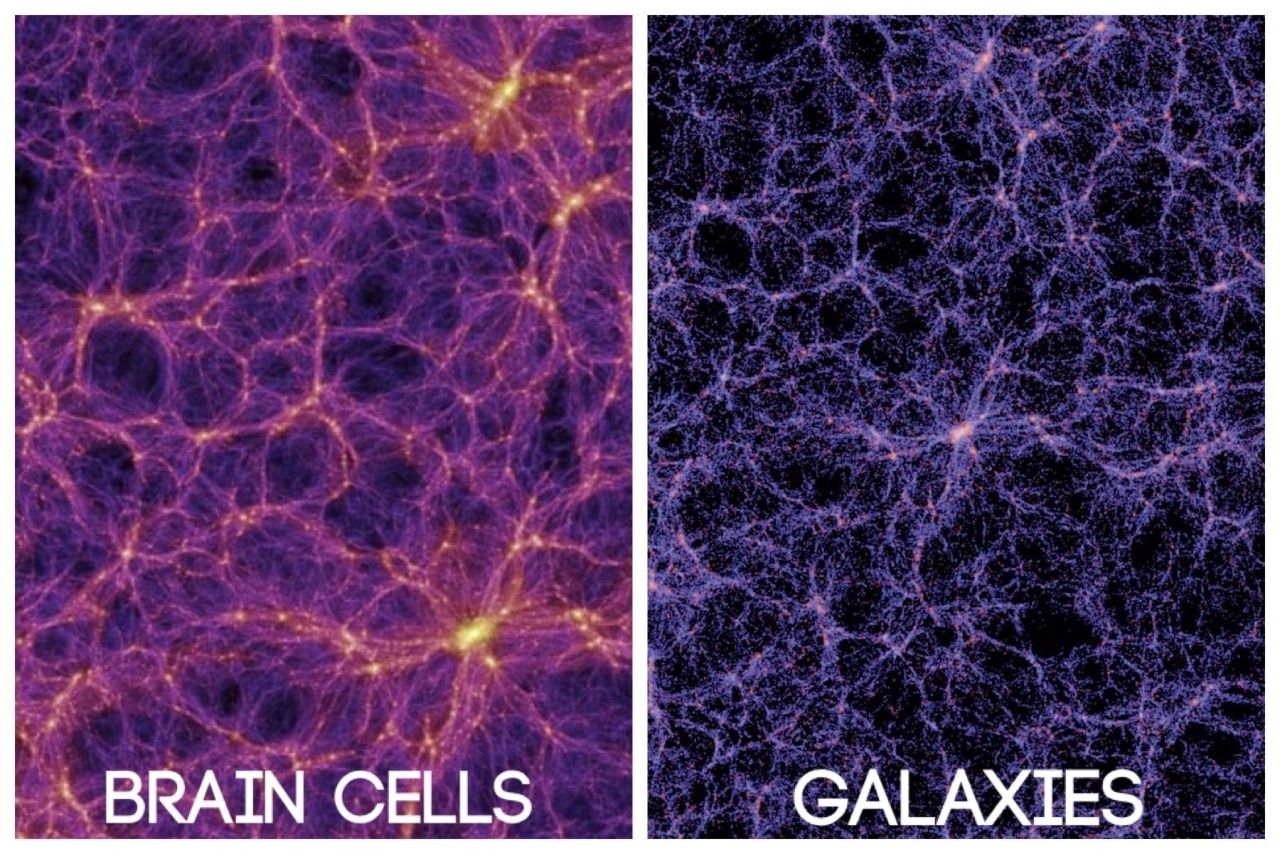
\includegraphics[scale=0.2]{komparacija.jpeg}
\end{center}
\caption{Komparacija ćelija mozga i galaksija}
\label{fig:komparacija}
\end{figure}

\justifying
Takođe, u oba sistema, ove mreže čine samo 30 \% mase. U svakom od njih oko 70 odsto mase zapravo čine delovi za koje se čini da su pasivni: moždana tečnost i tamna materija svemira.

Vitali Vančurin smatra da ukoliko posmatramo svemir kao neuronsku mrežu, njegovo ponašanje pod određenim uslovima možemo objasniti jednačinama kvantne mehanike i zakonima klasične fizike, poput teorije relativnosti koju je osmislio Albert Ajnštajn. Vačurin smatra da bi daljim proučavanjem ove teorije mogao rešiti glavni problem moderne fizike \--\ neslaganje klasične mehanike,
koja opisuje kako svemir funkcioniše u velikim razmerima i kvantne mehanike koja se bavi proučavanjem atomskog i subatomskog nivoa materije.  Kao što je poznato, razlika između klasične i kvantne mehanike jeste ta što je u klasičnoj mehanici vreme apsolutno i univerzalno, dok je u kvantnoj mehanici relativno.

 Vančurin je u intervjuu za časopis \textit{Futurism} \cite{7} istakao ključnu tačku svog rada. Naime, on je zaključio da je dinamika učenja neuronskih mreža veoma slična kvantnoj dinamici u fizici. Ono što je zapravo rečeno je da je učenje neuronskih mreža u nekim granicama logično, dok izvan tih granica ne važe ista pravila kao unutar njih. To se može uporediti sa zakonima klasične i kvantne mehanike. Najbolje bi to bilo predstaviti u tabeli \ref{tab:tabela1}


\begin{table}[h!]
\begin{center}
{\footnotesize
\begin{tabular}{|c|c|c|} \hline
 & Klasična fizika& Kvantna fizika\\ \hline
Svojstva& čestična ili talasna & i čestična i talasna\\ \hline
Pozicija i brzina& mogu se tačno odrediti& ne mogu se  tačno odrediti\\ \hline 
Dilatacija vremena& ne postoji & postoji \\ \hline
Kontrakcija dužine& ne postoji& postoji\\ \hline
\end{tabular}
\caption{Razlike između klasične i kvantne fizike}
\label{tab:tabela1}
}
\end{center}
\end{table}





\section{Neuronske mreže}
\label{sec:naslov1}
Neuronske mreže (eng. {\textit{neural networks}}) predstavljaju najpopularniju i jednu od najprimenjenijih metoda mašinskog učenja. Njihove primene su mnogobrojne i pomeraju domete veštačke inteligencije, računarstva i primenjene matematike. Neke od njih su:
\begin{itemize}
  \item kategorijzacija teksta
  \item medicinska dijagnostika
  \item prepoznavanje objekata na slikama
  \item autonomna vožnja
  \item igranje igara poput igara na tabli (tavla i go) ili video igara
  \item mašinsko prevođenje prirodnih jezika
  \item modelovanje semantike reči prirodnog jezika i slično
\end{itemize}
Neuronske mreže zapravo predstavljaju parametrizovanu reprezentaciju koja može poslužiti za aproksimaciju drugih funkcija. Kao i u slučaju drugih metoda učenja, pronalaženje odgovarajućih parametara se vrši matematičkom optimizacijom nekog kriterijuma kvaliteta aproksimacije i može biti računski vrlo izazovno.

\begin{figure}[h!]
\begin{center}
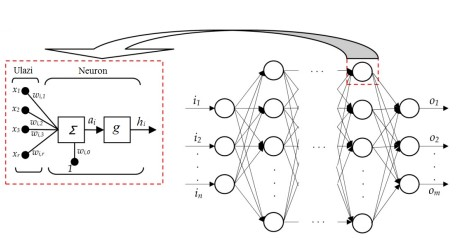
\includegraphics[scale=0.8]{fullyconnected.jpg}
\end{center}
\caption{Struktura potpuno povezane neuronske mreže.}
\label{fig:fullyconnected}
\end{figure}

Postoje različite vrste neuronskih mreža. Osnovnu varijantu predstavljaju potpuno povezane neuronske mreže (eng. {\textit{fully connected}}), koju možemo videti na slici \ref{fig:fullyconnected}. U obradi slika i drugih vrsta signala, pa i teksta, vrlo su popularne konvolutivne neuronske mreže (eng. {\textit{convolutional neural networks}}). Za obradu podataka nalik nizovima promenljive dužine, najčešće se koriste rekurentne neuronske mreže (eng. {\textit{recurrent nerual networks}}), a za obradu podataka koji se predstavljaju grafovima koriste se grafovske neuronske mreže (eng. {\textit{graph neural networks}}).

U svetlu njihovih izvanrednih uspeha i velike popularnosti, u laičkim krugovima postoji tendencija poistovećivanja mašinskog učenja, pa čak i veštačke inteligencije sa neuronskim mrežama. Ovakav pogled je prosto pogrešan. Takođe, postoji tendencija da se neuronska mreža razmatra kao prvi izbor metoda učenja nevezano od toga o kom se problemu radi. Ovo bi bio vrlo loš praktičan savet. Stoga naglašavamo u kakvim situacijama su superiorne u odnosu na druge modele. Dok je sasvim moguće da će neuronske mreže prestići druge modele i u drugačijim problemima, problemi zahvaljujući kojima su se neuronske mreže proslavile imaju određena zajednička svojstva. To su velika količina podataka i učenje na osnovu sirove reprezentacije podataka. Male količine podataka u slučaju neuronskih mreža lako vode preprilagođavanju neuronskih mreža, odnosno sposobnosti da same konstruišu nove atribute nad sirovom reprezentacijom podataka. Neuronske mreže su karakteristične po tome što su u stanju to da rade. Stoga, ukoliko je skup podataka mali nema razloga da očekujemo posebni benefit od primene neuronskih mreža, a moguće je da ćemo imati problema sa njihovim nedostacima. Ukoliko je veliki i u sirovom obliku, verovatno je dobra ideja primeniti neku varijaciju neuronske mreže.

\section{Vančurijev rad}

Godinama su fizičari pokušavali da pomire kvantnu mehaniku i opštu teoriju relativiteta. Kvantna mehanika tvrdi da je vreme apsolutno i univerzalno dok opšta teorija relativnosti tvrdi da je vreme relativno.

Vančurin tvrdi da neuronske mreže mogu da pokažu "približno ponašanje" obe teorije. Pošto je kvantna mehanika "izuzetno uspešna metodologija za modeliranje fizičkih pojava na širokom spektru skala", rasprostranjeno je verovanje da je na najosnovnijem nivou čitav univerzum vođen pravilima kvantne mehanike, pa da čak i gravitacija treba da izađe iz toga. On ne kaže samo da veštačke neuronske mreže mogu biti korisne za analizu fizičkih sistema ili za otkrivanje fizičkih zakona, već i da svet oko nas zapravo funkcioniše tako. U tom smislu to bi se moglo smatrati predlogom teorije svega, i kao takvo trebalo bi se dokazati da je pogrešno. 

Kako bi na jednostavniji način objasnio svoju teoriju, Vančurin je pokušao na dva načina pojasni svoje zaključke. Prvi način je da se počne sa preciznim modelom neuronskih mreža, a zatim da se proučava ponašanje mreže u granicama velikog broja neurona. Ono što je pokazao je to da jednačine kvantne mehanike prilično dobro opisuju ponašanje sistema blizu ravnoteže, a jednačine klasične mehanike opisuju kako je sistem dalje od ravnoteže. Drugi način je da krenemo od fizike. Znamo da kvantna mehanika radi jako dobro na malim razmerama, a opšta teorija relativiteta na velikim razmerama, no svakako nisu uspeli da pomire te dve velike teorije. Ovo je poznato kao pojam kvantne gravitacije. No to nije ni jedini problem, kako navodi Vančurin, već je i jedan od većih problema - problem posmatrača. S tim bi se moglo tvrditi da postoje tri fenomena koja treba objeniti. Većina fizičara bi reklo da je osnova kvantna mehanika i da nekako sve ostalo mora nastati iz nje, ali niko ne  zna kako. 

Vančurin je takođe sagledao mogućnost da je mikroskopska neuronska mreža osnovna struktura i da sve ostalo proizilazi iz nje. Do ideje je došao u jednom od svojih starih radova \cite{5}. Prvobitna ideja je bila da se metode statističke mehanike primene za proučavanje ponašanja neuronskih mreža, ali se pokazalo da je u određenim granicama dinamika učenja neuronskih mreža veoma slična kvantnoj dinamici koju vidimo u fizici. Tada je došao na ideju da je fizički svet zapravo neuronska mreža. Vančurin tvrdi da, kako bi se dokazalo da je ova teorija pogrešna, treba naći samo jedan fizički fenomen koji se ne može opisati neuronskim mrežama. Ovo je , naravno jako teško, jer ljudi jako malo znaju o tome kako se neuronske mreže ponašaju i kako mašinsko učenje zapravo funkcioniše. 

Vančurin nema ništa da kaže o tumačenju paralelnih univerzuma, ali navodi da može da doprinese teorijama skrivenih promenljivih. Skrivene promenljive su stanja pojedinačnih neurona, a promenljive koje se mogu obučiti su kvantne promenljive. Skrivene promenljive mogu biti nelokalne i time mogu narušiti Belove nejednakosti\footnote{ Bel je analizirao kvantno zapletanje mnogo dalje. On je zaključio da ako se merenja vrše nezavisno na dve odvojene čestice isprepletanog para, onda pretpostavka da ishodi zavise od skrivenih promenljivih unutar svake polovine implicira matematičko ograničenje na to kako su rezultati dva merenja povezani. Ovo ograničenje će kasnije biti nazvano Belova nejednakost.}.


\section{Istraživanja}
Pored Vančurija mnogi drugi naučnici bavili su se pitanjem svemira kao velike neuronske mreže. 

Kristof Koh (Christof Koch), koji je jedan od vodećih istraživača u oblasti svesti i ljudskog mozga, ljudski mozak je nazvao "najsloženijim objektom u poznatom svemiru". Ljudski mozak funkcioniše na osnovu razgranate neuronske mreže, dok svemir sadrži veliku mrežu od najmanje 100 milijardi galaksija. 

Dva italijanska naučnika Franko Vaza (Franco Vaca), astrofizičar, i Alberto Feleti (Alberto Feletti), neuronaučnik, u online časopisu \textit{Nautilus} iz 2018. godine opisali su sličnosti između neuronske i galaktičke mreže. 
\begin{itemize}
  \item svemir ima približan broj galaksija, koliko naš mozak ima ćelija (neurona) 
  \item kompjuterska simulacija kosmičke mreže i presek moždanog tkiva imaju sličnu strukturu 
  \item obe mreže imaju sličan spektar snage, koje daju sličan obrazac melodije za obe strukture 
  \item kosmička mreža i mozak imaju sličan stepen kompleksnosti, on se procenjuje merenjem veličine najmanjeg kompjuterskog programa koji može da predvidi ponašanje mreže (za kosmičku mrežu je broj od 1 do 10 petabajta (odnosno od 1000 do 10000 terabajta) podataka, dok je za ljudski mozak 2,5 petabajta), to bi značilo da se čitavo životno iskustvo jednog čoveka može kodirati u mrežu galaksija u svemiru
  \item autori su zaključili da su obe strukture, strukture koje se same organizuju
\end{itemize}

Donald Hofman (Donald Hoffman) postavio je osnovno pitanje o našim čulima. Da li nam ona govore istinu o stvarnosti? Hoffman smatra da otkad se pojavio Homo sapiens, prirodna selekcija je favorizovala percepciju koja skriva istinu i vodi nas prema korisnim radnjama, oblikujući naša čula. Donald je veliki prorok svesnog univerzuma. U njegovoj teoriji, najtemeljnija stvar je svesni faktor, a prostor-vreme i čestice samo su pojavna svojstva svesnog iskustva. 

U studiji objavljenoj u \textit{Nature’s Scientific Reports}, svemir raste na isti način kao i mozak. Simulacija razvoja svemira je traja 3,5 godine. Autori su zaključili da je prirodna dinamika rasta ista za različite vrste mreža (internet, mozak ili svemir). Jedan od glavnih autora Dmitri Krijukov, smatra da ovi svemir raste na isti način kao mozak deteta. Simulacija ranih faza razvoja svemira pokazala je ograničen rast u pojedinim segmentima, ali vrlo izražen u drugim. Sličan fenomen je prisutan u razvoju mozga. 

\section{Diskusija}
Entropijska kvantna mehanika je relativno nova \cite{4} oblast, ali oblast koja se brzo razvija \cite{5}. Glavni novi uvid je da kvantna mehanika možda nije fundamentalna teorija, već samo matematički alat koji omogućava izvođenje statističkih proračuna u određenim dinamičkim sistemima. Ako je to tačno, onda bi trebalo da se izvedu svi bitni elementi (kompleksna talasna funkcija, Šredingerova jednačina, itd.) iz prvog principa. U svom radu Vančurin radi upravo to za dinamički sistem neuronske mreže. Ovo pokazuje da neuronske mreže zaista mogu opisati kvantne pojave ali takođe i klasične pojave. 

Jedno od najkotroverznijih pitanja ovo teme je kako se makroskopski posmatrači mogu pojaviti u fizičkom sistemu. Pitanje je izuzetno važno ne samo za rešavanje nekih filozofskih debata, već i za razumevanje rezultata stvarnih fizičkih eksperimenata \cite{8} i kosmoloških posmatranja \cite{9}. Kao što je već pomenuto, naše trenutno razumevanje fundamentalne fizike ne dozvoljava nam da formulišemo samodoslednu definiciju posmatrača bez paradoksa i svakako vredi razmotriti mogućnost da su posmatrači fenomen koji se pojavljuje. Ako i kvantna mehanika i opšta relativnost nisu fundamentalni, već pojavni fenomeni, zašto onda i makroskopski posmatrači ne nastaju na neki način iz mikroskopske neuronske mreže. Ovaj zadatak Vančurin nije u potpunosti rešio ali daje jednu staru ideju koja bi ovde mogla biti relevantna. To je princip prirodne selekcije. Ne kosmološka prirodna selekcija \cite{10}, već biološka selekcija \cite{11}, iako bi to dvoje zapravo moglo biti povezano. Zaista ako je ceo univerzum neuronska mreža, onda bi se nešto poput prirodne selekcije moglo dešavati na svim skalama od kosmološke($>10^{15}$ m) i biološke($10^{2}-10^{-6}$ m) pa sve do subatomske($<10^{-15}$ m). Glavna ideja je da su neke lokalne strukture(ili arhitekture) neuronski mreža stabilnije na spoljne perturbacije(tj. interakcije sa ostatkom mreže) od drugih lokalnih struktura. Kao rezultat toga, veća je verovatnoća da će stabilnije strukture preživeti, a manje stabilne biti istrebljene. Nema razloga za očekivati da bi ovaj proces mogao biti ograničen na fiksnu skalu i stoga evolucija mora da se nastavi neograničeno na svim skalama. Ako je to tačno onda ono što sada nazivano atomima i česticama zapravo može biti rezultat duge evolucije počevši od nekih vrlo jednostavnih struktura. Naravno trenuto je tvrdnja da prirodna selekcija može biti relevantna na svim skalama veoma spekulativna ali izgleda da neuronske mreže nude zanimljivu novu perspektivu.
\section{Zaključak}

U ovom radu smo razmatrali mogućnost da je ceo univerzum na svom najosnovnijem nivou neuronska mreža. Ovo je veoma smela tvrdnja. Ne samo da kažemo da veštačke neuronske mreže mogu biti korisne za analizu fizičkih sistema \cite{2} ili za otkrivanje fizičkih zakona \cite{3}, već kažemo da svet oko nas zapravo funkcioniše tako. S tim na umu, to bi moglo smatrati predlogom teorije svega i kao takvo bi trebalo biti lako dokazati da je pogrešno. Sve što je potrebno je pronaći jedan fizički fenomen koji se ne može opisati neuronskim mrežama. Nažalost (ili na sreću), lakše je to reći nego učiniti. Pokazalo se da je dinamika neuronskih mreža toliko složena da se može razumeti samo u vrlo specifičnim granicama. Glavni cilj Vančurinovog rada bio je da se opiše ponašanje neuronskih mreža u granicama kada se relevantni stepeni slobode (kao što su vektor pristrasnosti, matrica težine, vektor stanja neurona) mogu modelovati kao stohastičke varijable koje prolaze kroz evoluciju učenja.

\printbibliography[
heading=bibintoc,
title={Literatura}
]

\end{document}
